\documentclass{article}
\usepackage[top=.5in, bottom=.5in, left=.9in, right=.9in]{geometry}
\usepackage[latin1]{inputenc}
\usepackage{enumerate}
\usepackage{hyperref}
\usepackage{graphics}
\usepackage{graphicx}
\usepackage{caption}
\usepackage{subcaption}
\usepackage{tabularx}
\usepackage{amsmath}
\usepackage{amssymb}
\usepackage{siunitx}
\usepackage{mathtools}

\newcommand{\obar}[1]{\ensuremath{\overline{ #1 }}}
\newcommand{\iid}{\ensuremath{\stackrel{\textrm{iid}}{\sim}}}

\usepackage{xcolor}
\definecolor{darkgreen}{rgb}{0,0.25,0}
\newcommand{\soln}{{\color{red}\textbf{Solution:~}\color{black}}}


\usepackage[formats]{listings}
\lstdefineformat{R}{~={\( \sim \)}}
\lstset{% general command to set parameter(s)
basicstyle=\small\ttfamily, % print whole listing small
keywordstyle=\bfseries\rmfamily,
keepspaces=true,
% underlined bold black keywords
commentstyle=\color{darkgreen}, % white comments
stringstyle=\ttfamily, % typewriter type for strings
showstringspaces=false,
numbers=left, numberstyle=\tiny, stepnumber=1, numbersep=5pt, %
frame=shadowbox,
rulesepcolor=\color{black},
,columns=fullflexible,format=R
} %
\renewcommand{\ttdefault}{cmtt}
% enumerate is numbered \begin{enumerate}[(I)] is cap roman in parens
% itemize is bulleted \begin{itemize}
% subfigures:
% \begin{subfigure}[b]{0.5\textwidth} \includegraphics{asdf.jpg} \caption{} \label{subfig:asdf} \end{subfigure}
\hypersetup{colorlinks=true, urlcolor=blue, linkcolor=blue, citecolor=red}


\graphicspath{ {C:/Users/Evan/Desktop/} }
\title{\vspace{-6ex}SDS385 HW 1\vspace{-2ex}}
\author{Evan Ott \\ UT EID: eao466\vspace{-2ex}}
%\date{DATE}
\setcounter{secnumdepth}{0}
\usepackage[parfill]{parskip}



\begin{document}
\maketitle
\section{Linear Regression}
\subsection{(A)}
WLS objective function:
\begin{align*}
\sum_{i=1}^N\frac{w_i}{2}(y_i-x_i^\top\beta)^2&=\frac{1}{2}\sum_{i=1}^Ny_iw_iy_i - \sum_{i=1}^Ny_iw_ix_i^\top\beta+\frac{1}{2}\sum_{i=1}^Nx_i^\top\beta w_ix_i^\top\beta\\
&=\frac{1}{2}y^\top W y - y^\top W X \beta + \frac{1}{2}(X\beta)^\top WX\beta\\
&=\frac{1}{2}(y-X\beta)^\top W(y-X\beta).
\end{align*}
Minimizing this function means setting the gradient (with respect to $\beta$) to zero:
\begin{align*}
\nabla_\beta\left[\frac{1}{2}(y-X\beta)^\top W(y-X\beta)\right]&=0
\end{align*}
That is
\begin{align*}
\nabla_\beta\left[\frac{1}{2}(y-X\beta)^\top W(y-X\beta)\right]&=0-(y^\top WX)^\top+\frac{2}{2}X^\top WX\hat{\beta}=0\\
&\Rightarrow (X^\top WX)\hat{\beta}=X^\top Wy~~~~_\blacksquare
\end{align*}

\subsection{(B)}
The matrix factorization idea basically amounts to trying to prevent the full inverse operation. Overall, you will still probably need something $O(n^3)$, but the constants matter when actually doing computation as opposed to asymptotics. We don't actually want the inverse anyway, we just want to solve $(X^\top WX)\hat{\beta}=X^\top Wy$ for $\beta$. Using a matrix
decomposition can help with that a lot.

I based my solution on the Cholesky decomposition (see \url{http://www.seas.ucla.edu/~vandenbe/103/lectures/chol.pdf}). This creates matrices $X=LL^\dagger$, where $L$ is lower-triangular. So, then solve $Lz=X^\top Wy$ for $z$ and $R\beta=z$ for $\beta$. The decomposition is still $O(n^3)$,
but faster than inverse. The two final steps are each $O(n^2)$ which are faster.

\subsection{(C)}
See code on GitHub (\texttt{matrix\_inverse\_functions.R} and \texttt{matrix\_inverse\_run.R}).

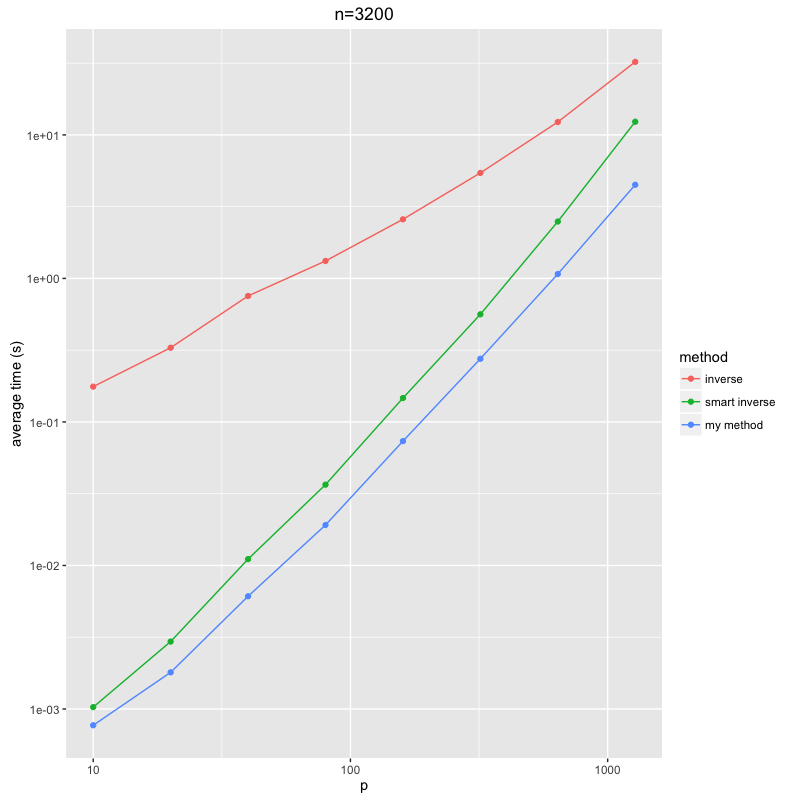
\includegraphics[scale=0.5]{log_methods.png}

\subsection{(D)}
See code on GitHub (\texttt{matrix\_inverse\_functions.R} and \texttt{matrix\_inverse\_run.R}, look for the ``Part D'' in each).

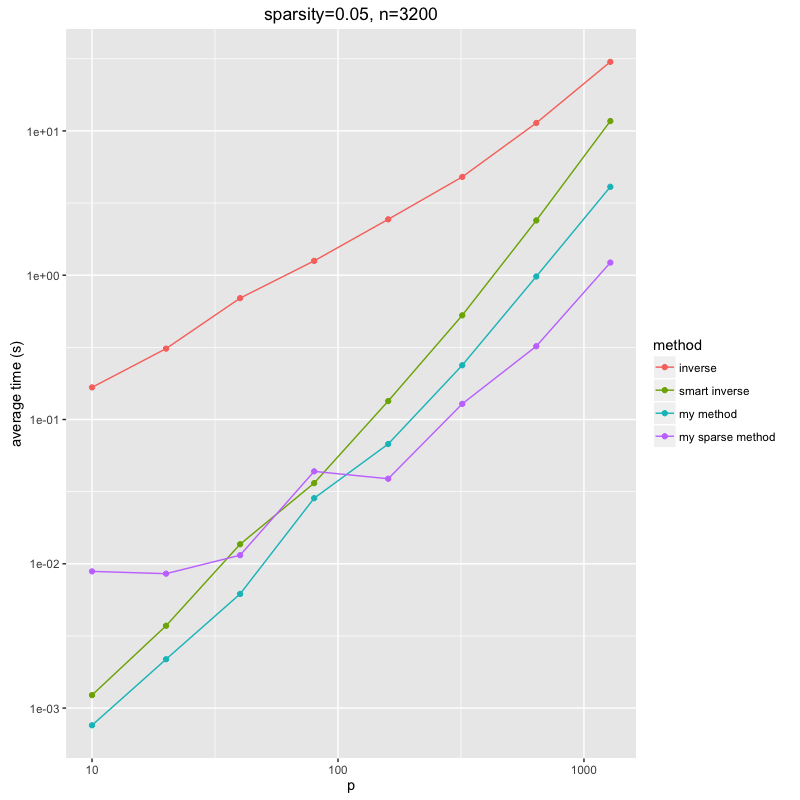
\includegraphics[scale=0.5]{sparse.png}

\subsection{Notes from class}
Three main matrix decomposition techniques:
\begin{enumerate}[1.]
\item Cholesky $\rightarrow$ fast, unstable (susceptible to roundoff error)
\item QR $\rightarrow$ middle ground
\item SVD $\rightarrow$ slow, but works for close-to-rank-deficient matrices
\end{enumerate}

Using QR, we get $W^{1/2}X=QR$, where $R$ is $P\times P$ and upper-triangular (and thus invertible) and $Q$ is $N\times P$ with
orthonormal columns.
\begin{align*}
X^\top Wy&=X^\top W X\beta\\
X^\top W^{1/2} W^{1/2}y&=X^\top W^{1/2}W^{1/2}X\beta\\
(QR)^\top W^{1/2} y&=(QR)^\top QR\beta\\
Q^\top W^{1/2}y&=I R\beta=R\beta\\
\end{align*}

A note on R, \texttt{crossprod} computes $X^\top X$ but recognizes the symmetry so it takes half the time.

High level: do \texttt{solve(A, b)} better than $x=A^{-1}b$.

Intermediate level: (where we want to be) factorize $A$ using a decomposition to not do the whole inverse. Especially
of note is whether we have sparse or dense matrices.

Low level: details of how the factorization works, what pivoting matrix to choose, etc.

Options for sparse matrices:
\begin{itemize}
\item Dictionary of keys
\item List of lists
\item Coordinate list (row, col, val)
\item Compressed sparse row format: $A$ stores non-zero elements, $AI$ is row info, $AJ$ is column indexes
\end{itemize}

\subsubsection{Example to try}
To see numerical precision, take a look at
\begin{align*}
\begin{pmatrix}10^{-5} & 1 \\ 1 & 1\end{pmatrix}
\begin{pmatrix} x_1\\x_2\end{pmatrix}
=
\begin{pmatrix}1\\0\end{pmatrix}
\end{align*}
using $LL^\top$ and QR decomposition with intermediate rounding (6 decimal places or so).

In terms of sparse matrix decomposition, try using sparse $LL^\top$ or sparse Cholesky, rather than QR because $Q$ will
not be sparse by definition, which makes all benefit be lost.


\section{Generalized linear models}
\subsection{(A)}
\begin{align*}
w_i(\beta)&=\frac{1}{1+\exp\{-x_i^\top\beta\}}\\
l(\beta)&=-\log\left\{\prod_{i=1}^N p(y_i | \beta)\right\}\\
&=-\log\left\{\prod_{i=1}^N \binom{m_i}{y_i} w_i(\beta)^{y_i} (1-w_i(\beta))^{m_i-y_i}\right\}\\
&=-\sum_{i=1}^N\log\left\{\binom{m_i}{y_i} w_i(\beta)^{y_i} (1-w_i(\beta))^{m_i-y_i}\right\}\\
&=-\sum_{i=1}^N\log\binom{m_i}{y_i} + y_i\log(w_i(\beta)) + (m_i-y_i)\log(1-w_i(\beta))\\
\nabla l(\beta)&=-\sum_{i=1}^N 0 + \frac{y_i}{w_i(\beta)} \nabla w_i(\beta) - \frac{m_i-y_i}{1-w_i(\beta)} \nabla w_i(\beta)\\
\nabla w_i(\beta)&=w_i^2(\beta) e^{-x_i^\top\beta} x_i\\
\nabla l(\beta)&=-\sum_{i=1}^N w_i^2(\beta) e^{-x_i^\top\beta} x_i\left(\frac{y_i}{w_i(\beta)}  - \frac{m_i-y_i}{1-w_i(\beta)}\right)\\
&=-\sum_{i=1}^N w_i^2(\beta) e^{-x_i^\top\beta} x_i\left(\frac{y_i-y_iw_i(\beta) - m_iw_i(\beta) + y_iw_i(\beta)}{w_i(\beta)(1-w_i(\beta))}\right)\\
&=-\sum_{i=1}^N w_i(\beta) e^{-x_i^\top\beta} x_i\left(\frac{y_i- m_iw_i(\beta)}{1-w_i(\beta)}\right)\\
&=-\sum_{i=1}^N w_i(\beta) \left(\frac{1}{w_i(\beta)} - 1\right)x_i\left(\frac{y_i- m_iw_i(\beta)}{1-w_i(\beta)}\right)\\
&=-\sum_{i=1}^N w_i(\beta) \frac{1-w_i(\beta)}{w_i(\beta)}x_i\left(\frac{y_i- m_iw_i(\beta)}{1-w_i(\beta)}\right)\\
&=-\sum_{i=1}^N \left[y_i- m_iw_i(\beta)\right]x_i\\
&=- X^\top(Y - Mw)
\end{align*}
where $M$ is a $N\times N$ diagonal matrix and $w$ is an $N$-vector with $M_{ii}=m_i$ and $w_i = w_i(\beta)$.

\subsection{(B)}
See code on GitHub (\texttt{glm.R} and \texttt{glm\_run.R}).

\subsection{(C)}
The second order Taylor approximation can be seen in Eq (2.14) in Nocedal \& Wright. First, we need the Hessian:

\begin{align*}
\nabla^2 l(\beta)=\nabla (\nabla l(\beta))&=\nabla_\beta\left(-\sum_{i=1}^N \left[y_i- m_iw_i(\beta)\right]x_i\right)\\
&=-\sum_{i=1}^N\left(\nabla_\beta\left[y_i- m_iw_i(\beta)\right]x_i\right)\\
&=-\sum_{i=1}^N\nabla_\beta\left(y_ix_i- m_iw_i(\beta)x_i\right)\\
&=\sum_{i=1}^Nm_i\nabla_\beta\left(w_i(\beta)x_i\right)\\
&=\sum_{i=1}^Nm_i\left(w_i(\beta)(1-w_i(\beta))x_i^\top x_i\right)\\
&=X^\top M W (I-W) X
\end{align*}
where $M$ and $W$ are $N\times N$ diagonal matrices with $M_{ii}=m_i$ and $W_{ii}=w_i(\beta)$.

Now, we can start computing the approximation. Let $\left(w_0\right)_i = w_i(\beta_0)$ and $\left(W_0\right)_{ii}=w_i(\beta_0)$, slightly modifying the previous results.

\begin{align*}
q(\beta; \beta_0)&= l(\beta_0) + (\beta-\beta_0)^\top \nabla_{\beta_0} l(\beta_0) + \frac{1}{2}(\beta-\beta_0)^\top \nabla_{\beta_0}^2 l(\beta_0) (\beta-\beta_0)\\
&=l(\beta_0) -  (Y - Mw_0)^\top X(\beta-\beta_0)+ \frac{1}{2}(\beta-\beta_0)^\top X^\top M W_0 (I-W_0) X (\beta-\beta_0)\\
&=l(\beta_0) +  (Y - Mw_0)^\top (X\beta_0-X\beta)+ \frac{1}{2}(X\beta_0-X\beta)^\top  M W_0 (I-W_0) (X\beta_0-X\beta)\\
A&=M W_0 (I-W_0)\\
b&=-A^{-1}(Y - Mw_0)\\
q(\beta; \beta_0)&=\frac{1}{2}(X\beta_0-b-X\beta)^\top A (X\beta_0-b-X\beta) + c(\beta_0)\\
z&=X\beta_0-b=X\beta_0+\left[M W_0 (I-W_0)\right]^{-1}(Y - Mw_0)\\
q(\beta; \beta_0)&=\frac{1}{2}(z-X\beta)^\top A (z-X\beta) + c(\beta_0)\\
\end{align*}

That is, $A$ is an $N\times N$ diagonal matrix and $z$ is an $N$-vector with:
\begin{align*}
A_{ii}&=m_i w_i(\beta_0) (1-w_i(\beta_0))\\
z_i&=x_i^\top\beta_0+\frac{Y_i-m_i w_i(\beta_0)}{m_i w_i(\beta_0) (1-w_i(\beta_0))}
\end{align*}


\subsection{(D)}
See code on GitHub (\texttt{glm.R} and \texttt{glm\_run.R}).

\subsection{(E)}
At least in my code, it seems that a couple things are true. First is that each iteration of the Newton's method is slower,
which makes sense because of the matrix inverse. However, based on my tests, it seems that even with a good multiplier, the steepest direction method doesn't attain as good as a result as the Newton method. Furthermore, the
steepest direction method took orders of magnitude more iterations to get to a reasonable result. In this case, it seems
like the Newton method is the way to go. But I'd imagine that with high-$P$, the inverse may be too expensive to perform.

\subsection{Notes from class}
Peer review likely due September 19.

For this problem, we have three kinds of convergence criteria:
\begin{enumerate}[1.]
\item an analytical criterion (for example, $\nabla l(\beta)=0$ known from the problem itself
\item when a sequence $\beta^{(1)},~\beta^{(2)},~\beta^{(3)},\ldots,\beta^{(n)}$ converges
\item $l(\beta^{(1)}),~l(\beta^{(2)}),~l(\beta^{(3)}),\ldots,l(\beta^{(n)})$ which is what almost all proofs use. It's the objective function and can be very flat near the optimum so it's better to use than $\beta$ on its own.
\end{enumerate}


\end{document}